
\documentclass{if-beamer}
\usepackage[utf8]{inputenc}			
\usepackage[russian]{babel}

\usepackage{tikz}			
\usepackage[T2A]{fontenc}




% --------------------------------------------------- %
%                  Титульник
% --------------------------------------------------- %
\title[ОГУ им. И.С.Тургенева.]{\textbf{Орловский Государственный университет им. И.С.Тургенева.}}
\author[Д.А. Селин]{\large \negrito{Д.А. Селин}}

\date{23 апреля 2025}
\logo{
\includegraphics[scale=0.8, clip]{figuras/logo.png}
}
% \subject{Presentation subject} % metadata
%trim={<left> <lower> <right> <upper>}
\graphicspath{{figuras/}}
% --------------------------------------------------- %
%                    Заголовок
% --------------------------------------------------- %


\begin{document}

\begin{frame}
  \titlepage
\end{frame}


\begin{frame}{ОГУ им. И.С.Тургенева}
  \frametitle{История университета}

  \noindent

  \begin{center}
      23 июня 1919 г. Образование Орловского пролетарского университета
  \end{center}

  \begin{figure}
      \centering
      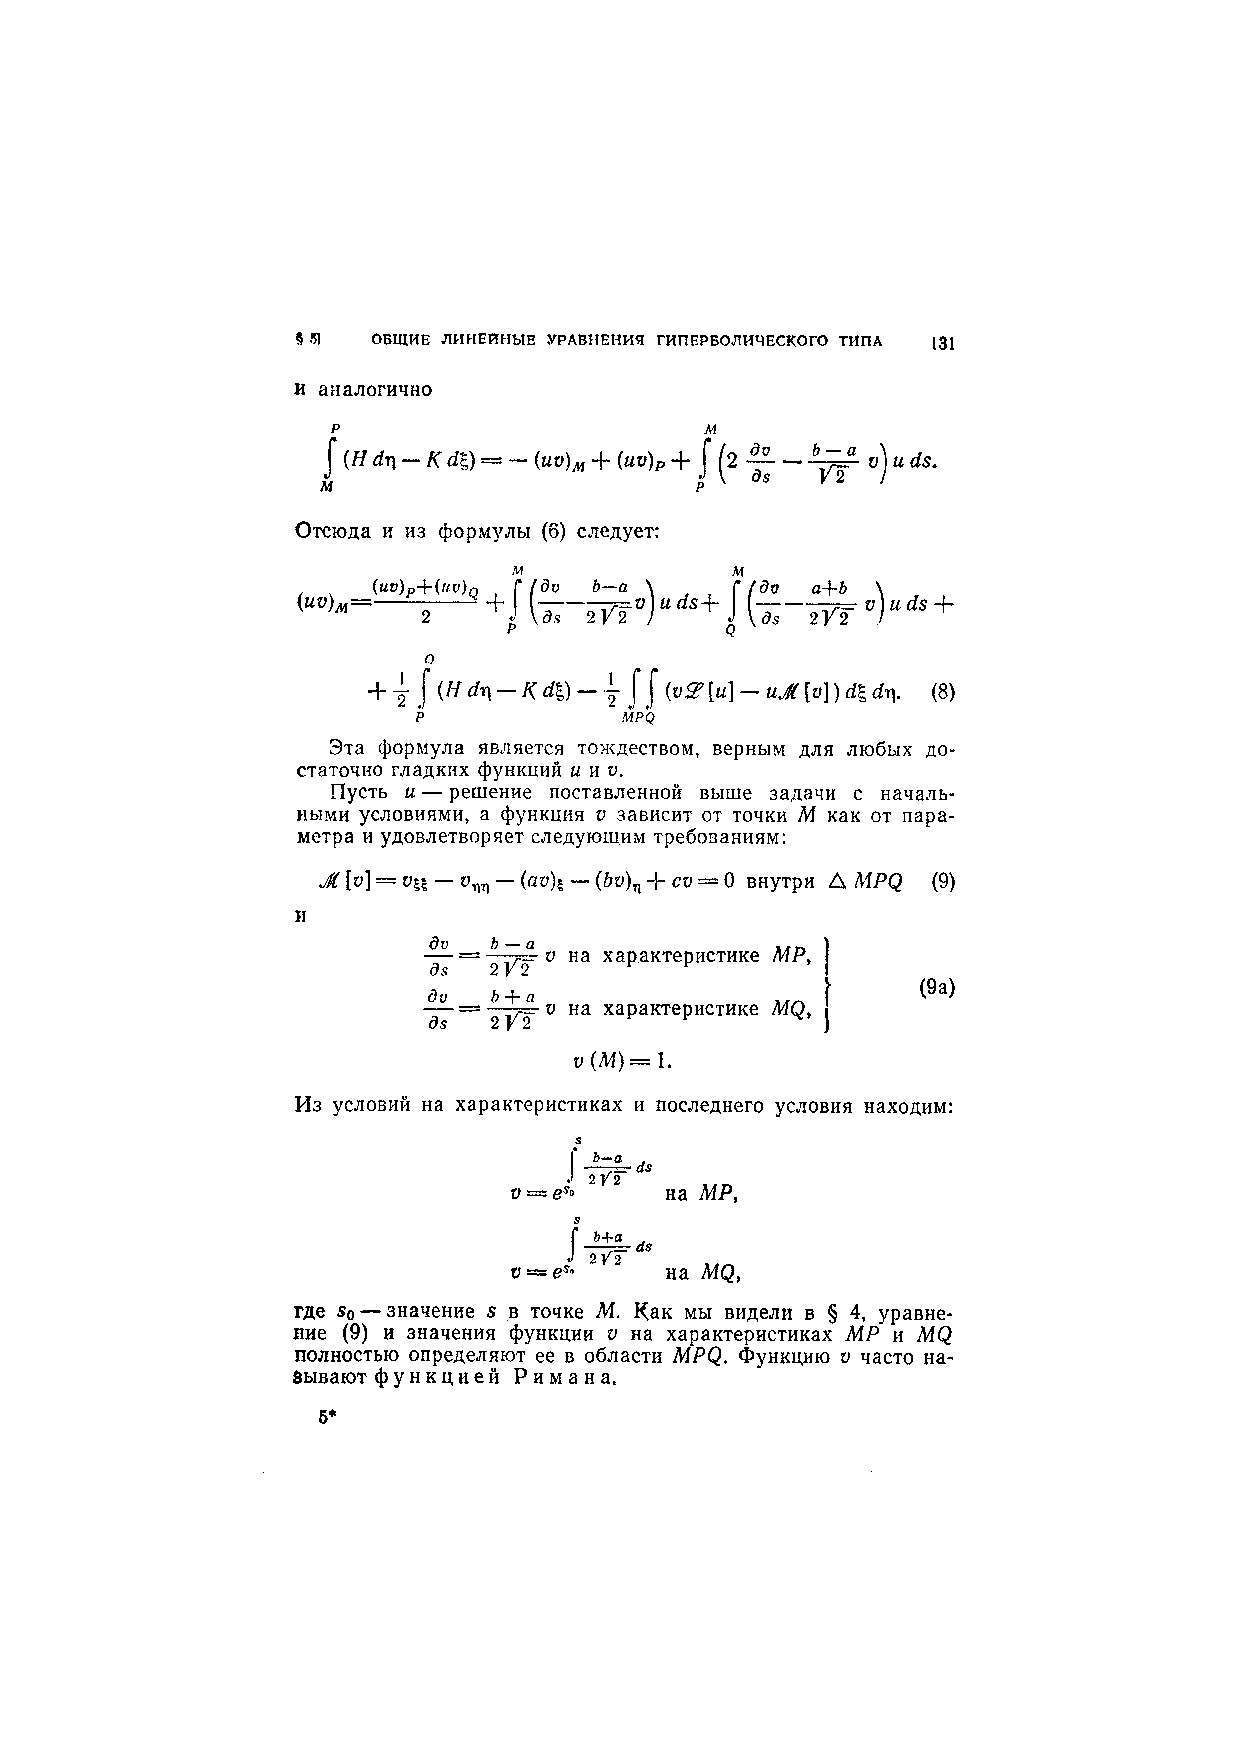
\includegraphics[width=0.7\linewidth]{figuras/1.jpg}
  \end{figure}
  \begin{center}
      В 1931 г. он стал индустриально-педагогическим институтом
  \end{center}
  
\end{frame}

\section{}

\subsection{}
\begin{frame}{ОГУ им. И.С.Тургенева}
    \frametitle{История университета}

    \begin{center}
        Институт открыл двери для 121 студента четырёх факультетов: Физ-мат, Хим-Био, Литературный, Политех.
    \end{center}

    \begin{figure}
        \centering
        \includegraphics[width=0.7\linewidth]{figuras/2.jpeg}
    \end{figure}

    \begin{center}
        11 Корпус ОГУ
    \end{center}

\end{frame}


\begin{frame}{ОГУ им. И.С.Тургенева}
\frametitle{Ректоры}

    \begin{center}
        2019 - 2024г. - А.А. Федотов
    \end{center}

    \begin{center}
        2025г. - Зомитева Г.М
    \end{center}

    \begin{figure}
        \centering
        \includegraphics[width=0.9\linewidth]{figuras/4-5.PNG}

    \end{figure}

\end{frame}

\begin{frame}{ОГУ им. И.С.Тургенева}
\frametitle{Награды университета}

    \begin{center}
       Университет получил орден "Знак Почёта"
    \end{center}

    \begin{figure}
        \centering
        \includegraphics[width=0.3\linewidth]{figuras/pochet.png}
    \end{figure}

\end{frame}

\subsection{}

\begin{frame}{ОГУ им. И.С.Тургенева}
\frametitle{События в истории}

    \begin{center}
        \begin{tabular}{|>{\centering\arraybackslash}m{2cm}|m{7cm}|}
          \hline
          \textbf{Дата} & \textbf{Событие} \\ \hline
          1933 год & Объединение с Белгородским педагогическим институтом \\ \hline
          1956 год & Педадогические высшие учебные заведения перешли на 5 летний план обучения \\ \hline
          18.08.2014 & ОГУ присвоено имя И. С. Тургенева \\ \hline
          28.10.2015 & Приказ об объединении ОГУ и ПГУ \\ \hline
        \end{tabular}
    \end{center}

    \begin{figure}
        \centering
        \includegraphics[width=0.5\linewidth]{figuras/7_1.PNG}
    \end{figure}

\end{frame}

\subsection{}
\begin{frame}{ОГУ им. И.С.Тургенева}
\frametitle{Заключение}

    \begin{center}
        На данный момент времени ОГУ является опорным вузом региона, который выпускает специалистов самых востребованных специальностей.
    \end{center}

    \begin{figure}
        \centering
        \includegraphics[width=0.8\linewidth]{figuras/10.PNG}

    \end{figure}

\end{frame}

\end{document}
